\documentclass[12pt,b5paper]{ltjsarticle}

\usepackage[margin=15truemm]{geometry}
\pagestyle{empty}

\usepackage{amssymb}
\usepackage{amsmath}	% required for `\align' (yatex added)






\usepackage{tikz}
\usetikzlibrary{calc}

\tikzset{set label/.style={fill=white,circle,inner sep=2}}

\def\radius{2}
\def\ratio{0.6}

\def\centerA{180:\ratio*\radius}
\def\centerB{0:\ratio*\radius}
\def\circleA{(\centerA) circle [radius=\radius]}
\def\circleB{(\centerB) circle [radius=\radius]}




\begin{document}

\begin{itemize}
 \item スペインが好きな人の中には、イタリアが好きな人もいる。
 \item スペインが好きな人は、すべてフランスも好きである。
\end{itemize}



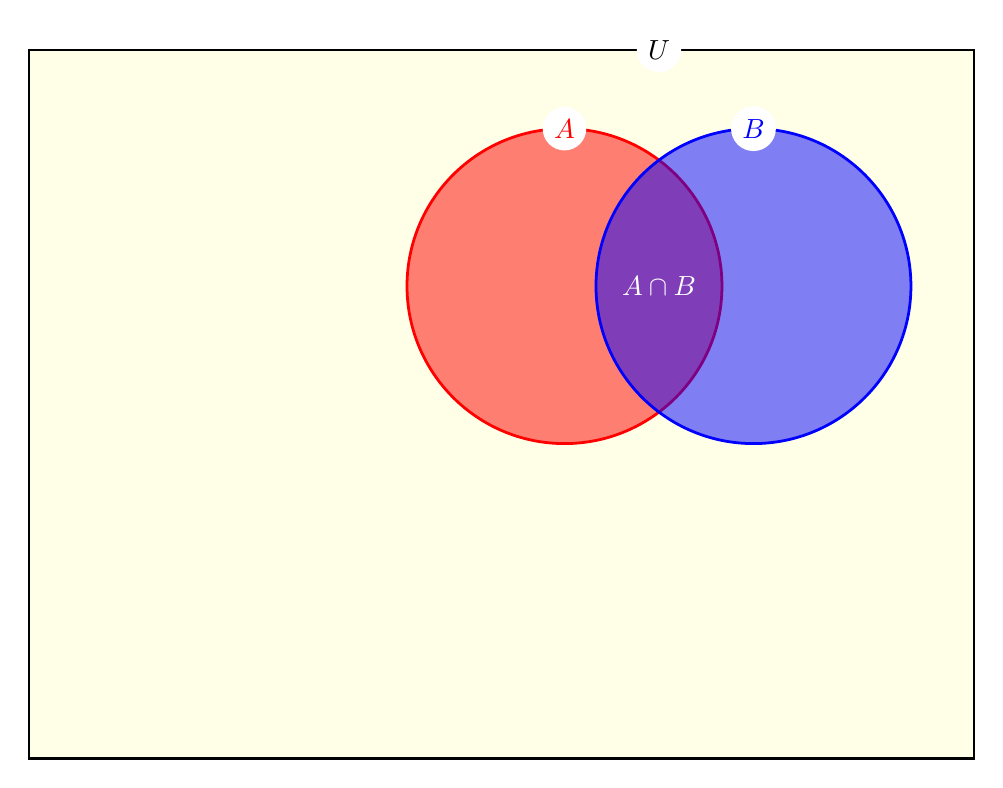
\begin{tikzpicture}
% 座標設定
\coordinate (O) at (0,0);
\coordinate (NE) at (4,3);
\coordinate (SW) at ($(O)!-2!(NE)$);
% 円の描画
\filldraw[draw=black, fill=yellow!10!white, line width=1pt] (SW) rectangle (NE);
\filldraw[draw=red, fill=red, fill opacity=0.5, line width=1pt] \circleA;
\filldraw[draw=blue, fill=blue, fill opacity=0.5, line width=1pt] \circleB;
% ラベルの描画
\node[set label] at (O |- NE) {$U$};
\node[set label,text=red] at ($(\centerA) + (90:\radius)$) {$A$};
\node[set label,text=blue] at ($(\centerB) + (90:\radius)$) {$B$};
\node[color=white] at (O) {$A\cap B$};
\end{tikzpicture}


\end{document}
